\chapter{Analysis}
\label{analysis}

\lettrine[lraise=0.1, nindent=0em, slope=-.5em]{\color{Violet}T}{his} chapter provides analytical part of the thesis beginning with analysis of the current situation following with analysis of the problems. Thereafter a requirement list for new e-course being established, followed by decision for methodology chosen for development of the e-course. 

\section{Problem Analysis}
\label{Problem Analysis}


Deficit of skilled \gls{ICT} specialist are known problem in Estonia \citep{website:ict_puudu} \citep{website:ict_needs}. However, several higher education institutes increased number of spots in \gls{ICT} curricula the outcome is insufficient \citep{website:TU_ict}, \citep{website:itc_facts}. Moreover, continuous changing and continuous learning are common in \gls{ICT} field. Therefore, a development of \gls{ICT} curriculum are continual activities in \gls{EITC} to maintain professionalism as a specialist.

During curriculum development process the \gls{EISA} contacted with \gls{EITC} describing a problem: The deficiency of the skilled and security aware system administrators and also provide initial proposal for solution as seen in Appendix~\ref{Letter from CERT.EE to the Rector of Estonian IT College} on page ~\pageref{Letter from CERT.EE to the Rector of Estonian IT College}. However, instead of accepting the solution without questioning we arranged several workshops for initial investigation of the problem and divided it to separate sub-problems and suggestions. For ensuring wider view of the problem several experts where involved from private companies, telecoms, banks, small business and start-ups.

First, many system administrators acquired their knowledge through self-study. However, a continuous study is common in \gls{ICT} field the level of the specialist are unsteady and they do not have sufficient knowledge to build secure infrastructure.

Second, the applied education field do not provide needed qualification needed to manage secure it infrastructure services.

Third, in retraining field is usual that private companies offer several courses for configuring and securing infrastructure, networks and services. However, those trainings are usually vendor based and focused heavily for promoting proprietary technologies.

Fourth, the system administrators in local government or municipal field constitute a whole with unevenly level of skills and knowledge. Therefore making maintaining and helping of the target group difficult for \gls{CERT.EE}.


Fifth, all courses (needed to be developed) should be associated with the practical applicability of the theoretical knowledge and contain largely practical hands-on classes. Moreover, all materials should be based on not proprietary technology, like \gls{OpenBSD} or \gls{GNU/Linux}.

Sixth, the study program should focuses on practical learning by doing approach to \gls{ICT} subjects. Moreover, using virtual and game-like environments is a contemporary approach for teaching IT System administration and programming focusing to the cyber security requirements increases a motivation of students. Today the studies include lectures, practical classes and independent work as homework. By and large, one subject is divided as follows: 25\% lectures, 25\% practical classes and 50\% homework which is mostly working with materials (books, web articles). In the worst case, practical work constitutes only 25\% and takes place at \gls{EITC} computer classes.
Moreover, the students are not interested in learning mere theory. The formulas are not seen necessary nor linked to their study area or future job. Theory that is not used will be forgotten quickly. In a few years students won't even remember if a specific topic was covered or not. Applied education should introduce practical approach and learning by doing. In ITC field practical classes and practical homework is the key to achieving acceptable results.
In initial investigation phase the authors role was curricula development, requirements management,  planning hands-on labs and course descriptions.


Designing an e-course is a challenge that has been solved by many lecturers and instructional developers. Moreover, the popularity of the cyber security related subjects in information and communications technology ICT curricula is growing and become a "student’s magnet" for higher educational institutes \citep{CyberIsHot}. Thereafter is possible to gain additional information by analysing related curricula in several higher educational institutes and analysing instructional design methodologies to achieve goals of this thesis.

\section{Related Work}
\label{Related Work}
Related Work...
ONE PAGE MAX
Panna siia lühikokkuvõte loetud teadusartikklitest IEEE*

Kauri magistritöö


\section{Choosing Methodology for Developing an e-course}

Developing a course instructions can proceeded using several methodologies. However, before choosing suitable approach for practical cyber security course some explanation of the terms e-course, e-learning, learning object, blended learning and hands-on laboratory classes are given to establish clear understanding for terminology used in thesis.

The term E-learning can be defined as the use of computer and Internet technologies to deliver a broad array of solutions to enable learning and improve performance \cite[p.~3]{food2011learning}.
V. Waller and J. Wilson 
E-course is a e-learning course and can be divided to one or several learning objects - {\color{red} TODO }

Learning object -  as a part of \gls{e-course} {\color{red} TODO }

Blended learning - {\color{red} TODO }

Hands-on laboratory - {\color{red} TODO }

Instructional design - {\color{red} TODO }

Today a learning by doing approach is accepted way to gain new skills and knowledge in cyber security field. This thesis focuses to develop of the practical hands-on e-course for system administrators in \gls{EITC}. Moreover the developed laboratories are used in higher education and also in continuous education classes.



\url{http://www.createdebate.com/debate/show/How_relevant_is_the_ADDIE_model_in_2009}

ADDIE model \url{http://www.youtube.com/watch?v=fdpHO1xycgo&list=PLEBAA915299F438EB}


Haridustehnoloogia sõnastik - \url{http://wiki.e-uni.ee/htsonastik/index.php?n=Main.Otilde#oppematerjal}

Miks creative common - \url{http://www.copyrightreform.eu/case-for-copyright-reform}

Alternative Training Models
Advances in Developing Human Resources November 2006 8: 460-475,


The methodology used to develop this e-course should encourage student activity in learning process. Moreover student should have possibility to choice learning speed, -place and -time. Today's students have different learning style and background and methodology should reckon with individual differences...

Developed e-course should support people with disabilities. In \gls{EITC} several people have hearing disabilities and all important material should presented also without audio. For example in screen casts videos all important information should be written also in screen or added as transcript.

Today’s learning environment should support student communities where students can act as mentors and also feel part on the study program. Course integration with student driven initiative like forums, blogs, wiki pages and other collaboration learning methods should be possible and not restricted.


Developing an e-course can be done without using design methodology but systematic approach should give more effective results. In principle the common systematic methods to develop an e-learning course are applying a Instructional System Design \gls{ISD} (sometimes cited as  Instructional Design \gls{ID}) model. However, several \gls{ISD} modes exists and can divided into three classes: behaviorism, cognitivist and prescriptive design \citep{website:id_models}, this thesis uses Prescriptive Design Model and specifically the \gls{ADDIE} process because method is used in Estonia and recommended for designing e-learning course \citep[p.~5]{OppeArenduskeskus2010}. However, the \gls{ADDIE} model has several weaknesses as \url{http://www.instructionaldesign.org/models/index.html}
For conclusion the \gls{ADDIE} model was chosen to develop cyber security e-learning course and model is described in the next section.

\subsection{The ADDIE Model}

The \gls{ADDIE} model is used for creating different types of instructions as courses, trainings \citep{website:addie}, \citep{lohr1998using}. Moreover, the ADDIE method is  used to provide a systematic, iterative course development process with feedback-based approach to improve quality of study \citep{website:using_addie}.

The ADDIE model contain five stages: Analysis, Desing, Development, Implementation and Evaluation as seen in illustration~\ref{figure:the addie model} \citep{website:addie}



\begin{figure}[H] 
 \centering 
 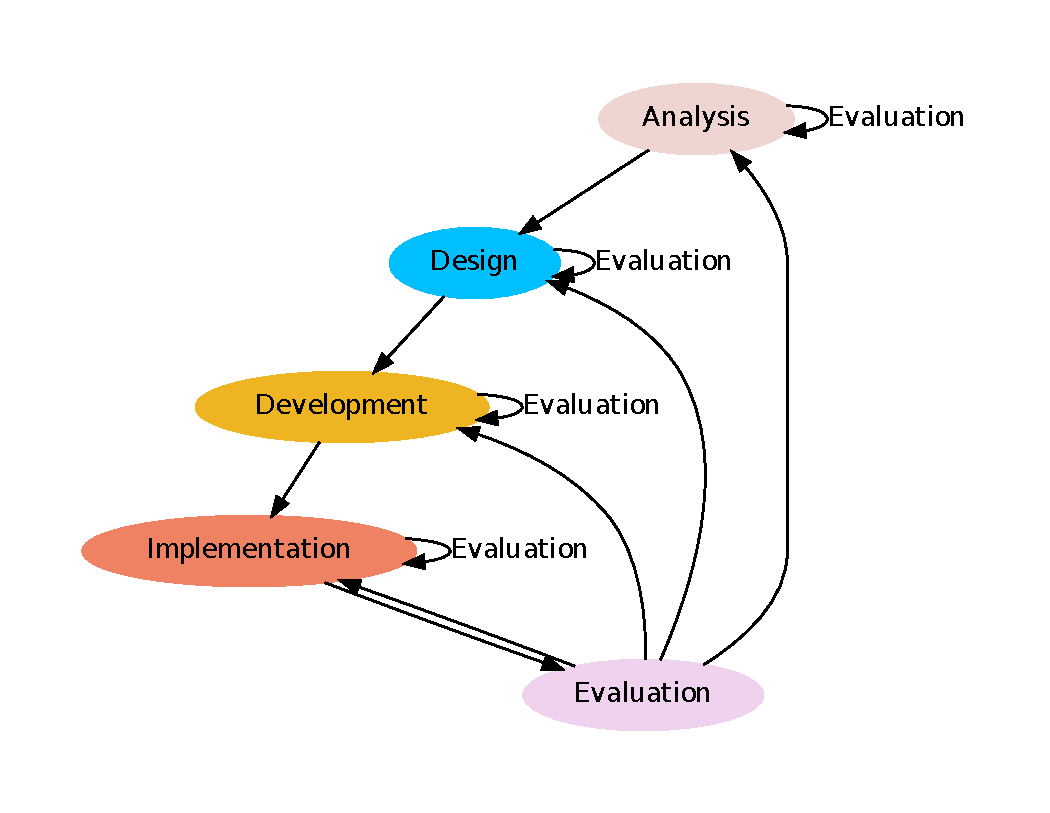
\includegraphics[width=0.9\textwidth]{addie_model.pdf}
 \rule{35em}{0.5pt} 
 \caption{The ADDIE model} 
 \label{figure:the addie model} 
\end{figure}

Firstly, the goal of the analysis phase is for investigation of the gap between goal and
existing situation. Therefore, this phase investigates instructional goals, current situation, learner, objectives \citep{chen2007learning} \citep{website:addie}.

Secondly, the design phase focuses following areas; assessments design, learning content, learning strategies and course format \citep{chen2007learning} \citep{website:addie}.


Thirdly, the work of development includes creating of course materials, choosing methodology and technologies, testing of material using run-through with small group. \citep{OppeArenduskeskus2010} \citep{website:addie} \citep{chen2007learning}.


Fourthly, the implementation stage is describes implementing the above work of three previous steps and gives possibility to evaluate full course in evaluation phase \citep{chen2007learning} \citep{website:addie}.


Finally, the evaluation phase is for assessing of the learning effect through evaluation. However the evaluation process takes place in every stage as seen in illustration~\ref{figure:the addie model} the final evaluation focuses whole course and focuses to the feedback from students and lecturers and output of this phase is valuable for next courses \citep{OppeArenduskeskus2010} \citep{website:addie}.



\section{Cyber security aspects of the e-learning}
Before starting instructional analysis of the e-learning course the cyber security aspect needs investigation to corrections and local modifications to the course development process. Therefore some questions need answer: Firstly, how studing cyber security affects student behaviour for example using learned methodologies to attack live systems? Secondly, does teaching in this field require special equipment comparing usual study of system administration? Thirdly, does field affect an usage of the methodology \gls{ADDIE} model chosen?

{\color{red} Uurida erinevaid cyber kursuseid } 


\section{Analysis of the e-learning course}
According to \gls{ADDIE} model the analysis stage establishes goals for the course and evaluation of the current situation and strategy for implementing goals followed by analysis of the learners and the content of the course \citep{website:addie}

The analysis phase of the \gls{ADDIE} model contains four sub-phases \citep{website:addie}.
\begin{enumerate}
\item Instructional Goals
\item Instructional Analysis
\item Learner Analysis
\item Learning Objectives
\end{enumerate}


\subsection{Instructional Goals}
The Instructional Goals should be established to compose main plan for new course. \citep{website:addie}


{\color{red} *

Vajaduste analüüs kirjeldab, mida tudengid juba enne teavad/peavad teadma

Vajalike teadmiste, oskuste ja suhtumiste kindlakstegemine.

Tegeliku olukorra hindamine ja cap analysis

prioriteetide loomine


Vajaduste analüüsimise meetodid:
kirjanduse uurimine, vestlused ekspertidega,


Vaatlused ja küsitlused,


testid - olemasolevate teadmiste hindamiseks

rühmaarutelusid  - õppija vajaduste ja ootuste hindamiseks, õpieesmärkide kindlakstegemiseks.


Asukoht õppekavas

Seos teiste õppeainetega

vajalikud eelteadmised

}



The general goal of the e-learning course are: firstly, give an introduction of IT infrastructure services, secondly, give skills and knowledge for installing and configuring of IT infrastructure services, thirdly give knowledge and skills for protecting IT infrastructure services. Moreover, give knowledge and skills for documenting IT infrastructure services.











To achieve this goal the study focuses on hands-on practical classes combined with lecturers and seminars. Moreover, the special priority given to security aspects of the services.

To achieve maximum impact of the course all content and methodology are designed to be suitable in classroom learning and using e-learning or blended learning which is combination of e-learning and classroom activities. Moreover, materials are designed to support self-study in e-learning form.

The name of the new course: Securing IT Infrastructure Services. However the course is not yet included into curricula the subject program will be discussed on board in June 2013 and in case positive feedback the new course will be held on Spring 2014.



\subsubsection{Analysing of the requirements, scope and restrictions for e-course}
During several curricula development seminars author establishes requirements for this particular e-course according to input from partners like \gls{EISA}, students feedback, graduate students feedback and curricula analysis from other higher educational institutes and private training companies. {\color{red} TODO tuua ära seminaride protokollid või viidata erinevatele piltidele, mis seminaris joonistati...vaja mõelda}


The main requirements can be presented as following:

\begin{enumerate}[label=Requirement \arabic*.,leftmargin=*]
  \item Developed e-course must be usable for \gls{EITC} students and also in continuous education field for system administrators
  \item Course must contain pre-sessional entry course to GNU/Linux and should cover basics  of the OpenBSD/FreeBSD systems
  \item Course should contains main aspects of system administration and focus to the defence of the systems
  \item Developed course materials should released using Creative Commons \gls{CC-BY-SA} license
  \item Laboratory work should be as realistic as possible including needed infrastructure to run complex infrastructure services. Therefore required solution for set-up hands-on environment in class or home.
\end{enumerate}


\subsection{Instructional Analysis}
The Instructional Analysis should answer the question: What steps are necessary to achieve  established instructional goals and what tools are needed? \citep{website:addie}.

 - during all of the necessary steps to achive the instructional goals. What tools we need? Sõltuvusgraaf - See on keeruline osa!




{\color{red} TINGIMUSTE ANALÜÜS (lk 8)
Missugused raha ja muud ressursid on vajalikud kursuse arendamiseks.

Kas auditoorne või muud tüüpi koolitus.

Mis materjale saab kohandada, tõlkida/muuta

}






%
%{\color{red} 
%Usable to design a learner centric course instead of teacher centric. 
%
%\url{http://www.youtube.com/watch?v=zB92UMyYzKM}
%
%Course content - get attencion
%Ingeraction amoungs students
%Jugement 
%Student diversity - ebaühtlus
%Create a role played scenario
%Analyse the material.
%
%\url{http://www.youtube.com/watch?v=oRgLqEF-qAU}
%
%}



\subsection{Learner analysis}

Learner Analysis - mida nad juba oskavad? interview and survives Selle tulemusena hoiame aega kokku ja teeme kursuse efektivsemaks. 


{\color{red}
taustandmed - vanus, sugu, elukoht tööhõive, töökogemus.

Motivatsioon - õppimise eesmärgid, ootused, lootused ja kartused, kursuse seotus nende tööga.

õppimisvõimet - eelnev haridustee, e-õppe kogemused, arvamused, isiklikud huvid 

eelnevad teadmised - oskused, arvamused, isiklikud huvid jne...
\citep{OppeArenduskeskus2010}


Vastab küsimusele:

Kes on kursusel osalejad?

Millised on eeltadmised, vajadused ja oskused.

Kui suurt sihtrühma saab õpetada?

Milline on tehniline varustus ja oskused seda kasutada?

Kas kursuse alguses tuleb arendada õpioskuseid

\citep{OppeArenduskeskus2010}
}

Learning Objectives - what students should be able to do when ...
- skills 

- attitude

- knowledge

When a student completes this e-course, hi/she should be able to ....

Use strong verbs:
explain
report
describe
list
demonstrate
compare
calculate
analyse

utilize resources better






The analysis of the target group gives input to the course development because starting point of the course and difficulty level of the hands-on labs depends on the target group. According to problem analysis the target group can divided to two separate groups, the students who do not have long working experience and system administrators who have working experience in particular field but do not have degree or diploma in \gls{ICT} field or they are graduated several years ago.

The first target group are second and third years students who already mastered basics of operating systems, GNU/Linux administration, Windows administration. The second target group are system administrators with different practical background because deep specializing in enterprises. Common relevant (on course development point of view)  properties are described in Table~\ref{tab:targetgroup}
\begin{table}[h]
\centering
\caption{The target group properties}

\begin{tabular}{|p{4cm}|p{5cm}|p{5cm}|}
\hline 
\color{blue}
Property & \color{blue} Students & \color{blue} System Administrators \\ 
\hline 
Background & No or few working experience & Experience on one or more specialized field \\ 
\hline 
Motivation & To get diploma and work and knowledge/skills needed to protect \gls{ICT} systems & To get knowledge and skills to protect \gls{ICT} systems \\ 
\hline 
Time and possibilities & possible to do home work/reading & in practice can not do homework/readings efficiently  \\ 
\hline 
Previous knowledge &   &   \\ 
\hline 
Previous study experience & Good & Lesser \\ 
\hline 
Study Stile & Student's style (everything done little before deadlines) & All study should take place during contact hours  \\ 
\hline 
How {\color{red}{homogeenne}} the group are  & More flat & {\color{red}{ebaühtlane}} \\ 
\hline 
Previous experience in GNU/Linux & Present & Poor (only 10\%) passed the test  \\ 
\hline 
\end{tabular} 

\label{tab:targetgroup}
\end{table}

In this time no data about age and ... {\color{red} TODO mis jäi vaatluse alt välja} because of insufficient data. 



For conclusion to target group's analysis can be stated that course material should be suitable for both groups. First group the students have advantage because time for home readings. However the second group has advantage from work experience. Second group's problem is insufficient knowledge about GNU/Linux system and separate short auxiliary course about basic command line is needed before entering to the main course. However some system administrators do not need those course and need for additional course will decided using entry test developed during this thesis.

According to motivation the main focus of new e-course to give practical hands-on approach for protecting \gls{ICT} systems.


\subsection{Learning Outcomes}

{\color{red} 

Mahu analüüs. Kas on sobiva mahuga?

Vastav kursuse tasemele?

Asjakohane ja arusaadavalt esitatud?

eelteadmistest lähtuv.

loogiliselt järjestatud.

}
\subsubsection{Analysis of the course content}

\begin{enumerate}[label=Hands-on block \arabic*.,leftmargin=*]
  \item Pre-requirements courses
    \begin{enumerate}[label=LAB \arabic*.,leftmargin=*]
  	\item Operating system basics (one day)
  	\item Basic networking IPv4/IPv6, TCP/IP (one day)
  	\item GNU/Linux basics (and OpenBSD/FreeBSD basics) (2 days)
  	\item Scripting in BASH (2 days)
  	\item Scripting in Python (1.5 days)
  	\item Scripting in PowerShell (1.5 days)
  \end{enumerate}
  \item Root services
  \begin{enumerate}[label=LAB \arabic*.,leftmargin=*]
  	\item NTP (0.5 days)
  	\item DNS (2.5 days)
  	\item DHCP (one day)
  \end{enumerate}
  \item Web/File Services
    \begin{enumerate}[label=LAB \arabic*.,leftmargin=*]
    \item Web server basics - installation of apache2 web server
  	\item Web server security - Protecting Web Application Against
(D)DOS Attacks
  	\item Web server security - securing vulnerable web application using application firewalls (3 days)
  	\item Fileserver (Samba3 and Samba4) (0.5 day)
  \end{enumerate}
    \item E-mail services (4 days)
    \begin{enumerate}[label=LAB \arabic*.,leftmargin=*]
  		\item SPAM control
	  	\item Virus protection
  		\item MTA's 
	  	\item MDA's
    \end{enumerate}
    \item IP firewalls and IDS/IPS (4 days)
        \begin{enumerate}[label=LAB \arabic*.,leftmargin=*]
  		\item IP firewalls netfilter/iptables and packet filter (pf) (2 days)
	  	\item IDS/IPS (2 days)
  		\item NetFlow (kuna seda loetakse CERT.EE abil, siis jääb välja)
    \end{enumerate}
    \item Autentication and authorization (4 days)
        \begin{enumerate}[label=LAB \arabic*.,leftmargin=*]
  		\item LDAP and Samba4 AD
	  	\item Windows and Linux clients with Samba4 AD 
  		\item Web application authentication with Samba4 AD and LDAP
    		\end{enumerate}
    \item GNU/Linux central management with Puppet
        \begin{enumerate}[label=LAB \arabic*.,leftmargin=*]
	  		\item Installation of Puppet using passenger (2 day)
		  	\item Writing puppet recipes (1 day)
    		\end{enumerate}
    	\item Central logging (3 days)
    	    \begin{enumerate}[label=LAB \arabic*.,leftmargin=*]
	  		\item Collecting logs with rsyslog/syslog-ng (1 day)
		  	\item Monitor and analyse log files (1 day)
    		\end{enumerate}
\end{enumerate}

Content can presented in several ways using {\color{red} lugeda Rowntree, D. Teaching through self-instruction: a practical handbook for course developers.} \citep{rowntree1986teaching}


\section{Design and Planning of learning process}

The Design phase contains three steps: First Design Assessments, second choose a course format, third create an instructional strategy.

Design assessments before creating a content - nagu tagant ettepoole minek.

Assessment design contains (goals, lerners, context, assessment)
kõiki õpiväljundeid tuleb testida.
assessments: clearly written, correct punctuation and grammar.

Choosing a course format is a delivery system like medium used to present the course.
- classroom
- e-course
- blended -combines different methods
- 

Instructional strategy
Collection of 
-lectures
-readings
-discussions
-projects
-worksheets
-assessments
-activities
Activities can be divided into five topics
\begin{enumerate}
\item Pre-instructional activities (motivate the students, mida nad pärast paremini teha oskavad, peale seda presenteerida objectives)
\item Content Presentation (consice content - no too many details, examples, )
\item Learner Participation (practice and feedback, )
\item Assessment (lisaks final assesment, practical assesment, attitude assesment  - ask students how thei feel about course )
\item Follow-through activities (review of entire course strategy .. veidi segane)
\end{enumerate}



Two possible e-learning processes are common the self-paced and facilitated/instructor-led \citep[p.~10]{food2011learning}.

Do we use collaboration in learning? 

Do we use  e-tutoring, e-coaching, e-mentoring?

Do we use chronological order or problem based? (one is good for lecturing other for practical classes) Also possible ways is spiral order logical order etc {\color{red} (viidata) }

Is the content sufficient to gain learning outcomes?

Is amount of work and student workload normal? How many academic hours for practical classes and home reading/lectures?

\subsection{Pedagogical view of the e-course}
Different Pedagogical strategies can be used during learning process. First a problem based approach is {\color{red} Pooleli }
Second koostööl põhinev õpe ja kolmas kogukonnal põhinev õpe.

Do we use group-work, wiki, blog and/or some e-learning environment?

Synchronous or asynchronous learning.

\subsection{Planning grading/assessment techniques}
What grading methods are useful for this particular course?

Do we need grade knowledge, skills and {\color{red} Pooleli }

Several assessment methods are used to give feedback and grades for students in e-courses {\color{red} Viide+listile viide }

\begin{itemize}
	\item self-assessment
	\item computer assessment
	\item tutor assessment
	\item peer assessment
\end{itemize}
\subsection{Choosing technological tools}
Keywords to focus {\color{red} Viidata }
\begin{itemize}
	\item availability
	\item usability 
	\item motivating students
	\item adaptive methods
	\item standard compliance
\end{itemize}
\subsubsection{E-Learning platforms}

\begin{itemize}
	\item Millal e-õpe töötab ja millal ei? Õppur peab rohkem pingutama [Chao: 11]
	\item Erinevad õpikeskkonnad ja nende sobivus antud õppeks
		\begin{itemize}
			\item Moodle
			\item Blackboard WebCT
			\item CISCO Network Academy
			\item Maurus
			\item IVA
			\item Sakai
			\item Wikiversity
			\item TUT Kaur course lab
		\end{itemize}
	\item virtual distance laboratory
	\item security aspects of distance laboratory
\end{itemize}



